\documentclass[a4paper, oneside]{book}
% Some basic packages
\usepackage[utf8]{inputenc}
\usepackage[T1]{fontenc}
\usepackage{textcomp}
\usepackage[english]{babel}
\usepackage{url}
\usepackage{graphicx}
\usepackage{float}
\usepackage{booktabs}
\usepackage{enumitem}
\usepackage[a4paper, margin=1.5cm]{geometry}

\pdfminorversion=7

% Don't indent paragraphs, leave some space between them
\usepackage{parskip}

% Hide page number when page is empty
\usepackage{emptypage}
\usepackage{subcaption}
\usepackage{multicol}
\usepackage{xcolor}

% Other font I sometimes use.
\usepackage{cmbright}


% Math stuff
\usepackage{amsmath, amsfonts, mathtools, amsthm, amssymb}
% Fancy script capitals
\usepackage{mathrsfs}
\usepackage{cancel}
% Bold math
\usepackage{bm}
% Some shortcuts
\newcommand\N{\ensuremath{\mathbb{N}}}
\newcommand\R{\ensuremath{\mathbb{R}}}
\newcommand\Z{\ensuremath{\mathbb{Z}}}
\renewcommand\O{\ensuremath{\emptyset}}
\newcommand\Q{\ensuremath{\mathbb{Q}}}
\newcommand\C{\ensuremath{\mathbb{C}}}

\addto\captionsenglish{% Replace "english" with the language you use
  \renewcommand{\contentsname}%
    {Lectures Index}%
}
% Easily typeset systems of equations (French package)
\usepackage{systeme}

% Put x \to \infty below \lim
\let\svlim\lim\def\lim{\svlim\limits}

%Make implies and impliedby shorter
\let\implies\Rightarrow
\let\impliedby\Leftarrow
\let\iff\Leftrightarrow
\let\epsilon\varepsilon

% Add \contra symbol to denote contradiction
\usepackage{stmaryrd} % for \lightning
\newcommand\contra{\scalebox{1.5}{$\lightning$}}

% \let\phi\varphi

% Command for short corrections
% Usage: 1+1=\correct{3}{2}

\definecolor{correct}{HTML}{009900}
\newcommand\correct[2]{\ensuremath{\:}{\color{red}{#1}}\ensuremath{\to }{\color{correct}{#2}}\ensuremath{\:}}
\newcommand\green[1]{{\color{correct}{#1}}}

% horizontal rule
\newcommand\hr{
    \noindent\rule[0.5ex]{\linewidth}{0.5pt}
}

% hide parts
\newcommand\hide[1]{}

% si unitx
\usepackage{siunitx}
\sisetup{locale = FR}

% Environments
\makeatother
% For box around Definition, Theorem, \ldots
\usepackage{mdframed}
\mdfsetup{skipabove=1em,skipbelow=0em}
\theoremstyle{definition}
\newmdtheoremenv[nobreak=true]{definition}{Definition}
\newtheorem*{eg}{Example}
\newtheorem*{notation}{Notation}
\newtheorem*{previouslyseen}{As previously seen}
\newtheorem*{remark}{Remark}
\newtheorem*{note}{Note}
\newtheorem*{problem}{Problem}
\newtheorem*{observe}{Observe}
\newtheorem*{property}{Property}
\newtheorem*{intuition}{Intuition}
\newmdtheoremenv[nobreak=true]{prop}{Proposition}
\newmdtheoremenv[nobreak=true]{theorem}{Theorem}
\newmdtheoremenv[nobreak=true]{corollary}{Corollary}

% End example and intermezzo environments with a small diamond (just like proof
% environments end with a small square)
\usepackage{etoolbox}
\AtEndEnvironment{vb}{\null\hfill$\diamond$}%
\AtEndEnvironment{intermezzo}{\null\hfill$\diamond$}%
% \AtEndEnvironment{opmerking}{\null\hfill$\diamond$}%

% Fix some spacing
% http://tex.stackexchange.com/questions/22119/how-can-i-change-the-spacing-before-theorems-with-amsthm
\makeatletter
\def\thm@space@setup{%
  \thm@preskip=\parskip \thm@postskip=0pt
}


% Exercise 
% Usage:
% \oefening{5}
% \suboefening{1}
% \suboefening{2}
% \suboefening{3}
% gives
% Oefening 5
%   Oefening 5.1
%   Oefening 5.2
%   Oefening 5.3
\newcommand{\oefening}[1]{%
    \def\@oefening{#1}%
    \subsection*{Oefening #1}
}

\newcommand{\suboefening}[1]{%
    \subsubsection*{Oefening \@oefening.#1}
}


\usepackage{xifthen}
% \def\testdateparts#1{\dateparts#1\relax}
% \def\dateparts#1 #2 #3 #4 #5\relax{
%     \marginpar{\small\textsf{\mbox{#1 #2 #3 #5}}}
% }

\usepackage{tocloft}

\newcommand{\cftchapterdotsep}{\cftdotsep}
\renewcommand{\cftchapleader}{\cftdotfill{\cftchapterdotsep}}

\newcommand{\currentcourse}{} 
\newcommand{\course}[1]{%
    \gdef\currentcourse{#1}%
}

\def\@lecture{}%
\newcommand{\lecture}[3]{%
    \ifthenelse{\isempty{#3}}{%
        \def\@lecture{Lecture #1}%
        \def\@lecturenum{#1}%
        \def\@lecturetitle{#3}%
        \addcontentsline{toc}{chapter}{Lecture #1}%
        \chapter*{\small{#2}\\\LARGE{Lecture #1}}%
        \markboth{}{Lec #1}%
        \thispagestyle{fancy}%
        \gdef\currentlecture{Lec #1}%
    }{%
        \def\@lecture{Lecture #1: #3}%
        \def\@lecturenum{#1}%
        \def\@lecturetitle{#3}%
        \addcontentsline{toc}{chapter}{Lecture #1: #3}%
        \chapter*{\small{#2}\\\LARGE{Lecture #1 - #3}}%
        \markboth{}{Lec #1 - #3}%
        \thispagestyle{fancy}%
        \gdef\currentlecture{Lec #1 - #3}%
    }%
}


\usepackage{tocloft}
\renewcommand{\cftsecleader}{\cftdotfill{\cftdotsep}}

\usepackage{fancyhdr}
\setlength{\headheight}{20pt}
\pagestyle{fancy}
\fancyhf{}
\fancyhead[L]{\currentcourse}
\fancyhead[R]{\currentlecture}
\fancyfoot[C]{\thepage}
\renewcommand{\headrulewidth}{0.4pt}
\renewcommand{\footrulewidth}{0pt}

\usepackage{todonotes}
\usepackage{tcolorbox}

\tcbuselibrary{breakable}

\newenvironment{correction}{\begin{tcolorbox}[
    arc=0mm,
    colback=white,
    colframe=green!60!black,
    title=Opmerking,
    fonttitle=\sffamily,
    breakable
]}{\end{tcolorbox}}

\newenvironment{notebox}[1]{\begin{tcolorbox}[
    arc=0mm,
    colback=white,
    colframe=white!60!black,
    title=#1,
    fonttitle=\sffamily,
    breakable
]}{\end{tcolorbox}}


\usepackage{import}
\usepackage{xifthen}
\usepackage{pdfpages}
\usepackage{transparent}
\newcommand{\incfig}[1]{%
    \def\svgwidth{\columnwidth}
    \import{./figures/}{#1.pdf_tex}
}

% Fix some stuff
% %http://tex.stackexchange.com/questions/76273/multiple-pdfs-with-page-group-included-in-a-single-page-warning
\pdfsuppresswarningpagegroup=1

\author{Ash Stewart}
\date{Semester 1}
\title{Lecture Notes}
\begin{document}
    \begin{titlepage}
        \maketitle
    \end{titlepage}
    \tableofcontents

    \part*{LC Classical Mechanics and Relativity 1}
    \addcontentsline{toc}{part}{LC Classical Mechanics and Relativity 1}
    \graphicspath{{Classical Mechanics and Relativity 1/}}
    \course{LC Classical Mechanics and Relativity 1}
    % start lectures CMR1
    % !TeX root = master.tex

\lecture{1}{Wed 01 Oct 2025 11:00}{Intro to Waves and SHM Recap}

\subsection*{Course Objectives}
\begin{itemize}
    \item Have a sound understanding of basic wave properties
    \item Have a basic understanding of interference effects, inc diffraction
    \item Be able to use simple geometric optics and understand the fundamentals of optical instruments.
\end{itemize}


\subsection*{Recommended Textbooks}
\begin{enumerate}
    \item University Physics, Young and Freedman (Ch 15, 16 for Waves, Ch 33-36 for Optics)
    \item Physics for Scientists and Engineers (Ch 20, 21 for Waves, Ch 22-24 for Optics)
    \item 5e, Tipler and Mosca, (Ch 15, 16 for Waves, 31-33 for Optics)
    \item Fundamentals of Optics, Jenkins and White
    \item Optics, Hecht and Zajac
\end{enumerate}

\paragraph{What is a wave?} Waves occur when a system is disturbed from equilibrian and the disturbance can travel from one region to another region. Waves carry energy, but do not move mass. The course aim is to derive basic equations for describing waves, and learn their physical properties.

\subsection*{Periodic Motion}
Waves are very linked to periodic motion. Therefore we recap periodic motion first.

It has these characterstics:
\begin{itemize}
    \item A period, $T$ (the time for one cycle)
    \item A frequency, $f$, the number of cycles per unit time ($f = \frac{1}{T}$)
    \item An amplitude, $A$, the maximum displacement from equilibrium.
\end{itemize}

Periodic motion continues due to the restoring force. When an object is displaced from equilibrium, the restoring force acts back towards the equi point. The object reaches equi with a non-zero speed, so the motion continues past the equi point and continues forever.

\subsection*{Energy}
Periodic motion is an exchange between potential and kinetic energy, with no energy loss. Energy is conserved.

\subsection*{Simple Harmonic Motion}
If the restoring force is directly proportional to the displacement $F = -kx$, then the periodic motion becomes Simple Harmonic Motion and the object is called a harmonic oscillator.

In a single dimension, displacement is given by:
\[
    x = A \cos(\omega t + \phi)
\]
Where $\omega = 2 \pi f$ is the angular velocity, and $\phi$ is the phase angle. In cases like this, where the phase angle is $90 \deg$ we can simplify to $x = A \cos(\omega t)$
\begin{figure}[H]
    \centering
    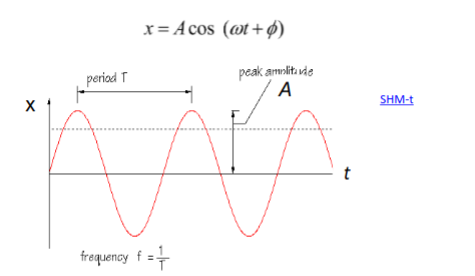
\includegraphics{figures/phaseangle.png}
    \caption{A Phase Angle of 90}
\end{figure}

\subsection*{More SHM Equations}
\textbf{Velocity}

\[
    v_x = \frac{dx}{dt} = - \omega A \sin(\omega t + \phi)
\]

\textbf{Acceleration}

\[
    a_x = \frac{d v_x}{dt} = \frac{d^2 x}{dt^2} = - \omega^2 A \cos(\omega t + \phi)
\]

Both properties are signed to indicate direction, as they are both vectors.




    % !TeX root = main.tex
\lecture{2}{Fri 10 Oct 2025 12:00}{The Ultraviolet Catastrophe}

In this lecture:
\begin{itemize}
    \item How classical theories fail to explain black body radiation (``The Ultraviolet Catastrophe'').
    \item How quantising light into photons gives predictions that fit this observation.
\end{itemize}

\section*{Black Body Radiation}
A `black body' is an idealised perfect object, that does not reflect, and absorbs internally all light (regardless of wavelength) incident upon it. No light is transmitted, so nothing shines out the other side. The object is perfectly black.

All bodies emit electromagnetic energy, usually outside the visible portion of the spectrum. For example, Paul Hollywood (and other humans) emit at about 300 Kelvin, which is infrared (at the temperature which night vision goggles are tuned to).

For the black body, emission spectrum is \textbf{only} from this thermal emission (no reflection, no flourescence, etc). Hotter objects are brighter and bluer (hotter means higher energy, and therefore a shorter wavelength)

\begin{figure}[H]
    \centering
    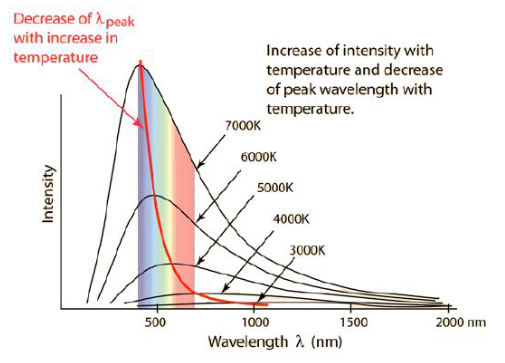
\includegraphics{figures/lec02-01.png}
     \caption{Observed Emission Spectra}
\end{figure}

However, we run into a problem. If we plot the spectra predicted by classical thermodynamics, vs the observed spectra for a given temperature object, the classical prediction gets it totally wrong, especially at shorter wavelengths.

\begin{figure}[H]
    \centering
    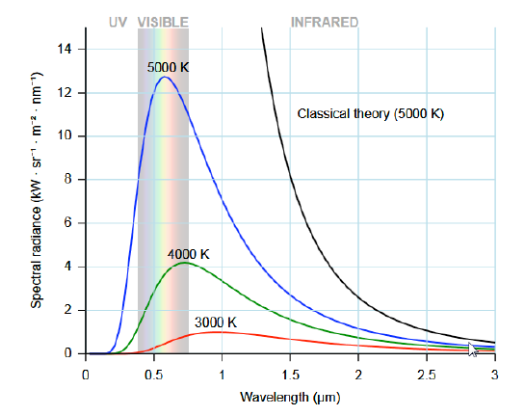
\includegraphics{figures/lec02-02.png}
     \caption{Predicted and Observed Spectra for 5000K (and Observed for 4k K and 3k K)}
\end{figure}

\subsection*{Notation}
$I(\lambda)$ is the intensity per wavelength for an emitted wavelength $\lambda$. $I$ is the total intensity across all wavelengths per unit time (in $W/m^2$, power per unit area).

\[
    I = \int_{0}^{\infty} I(\lambda) \, d \lambda
\]

I is the total area under the $I(\lambda)$ curve, i.e. the sum of intensity per wavelength, across every wavelength.

\section*{The Ultraviolet Catastrophe}
\subsection*{Empirical Results}
The Stefan-Boltzmann Law gives $I = \sigma T^4$, where $\sigma$ is the Stefan-Boltzmann constant, $\sigma = 6.57 \times 10^{-8} W m^{-2} K^{-4}$

Wien's Displacement Law gives $\lambda_{\text{peak}} = \frac{b}{T}$, where $b = 2.898 \times 10^{-3} Km$.

\subsection*{Why does classical mechanics break?}

Lets model the $I(\lambda)$ spectrum by slotting standing waves into a cavity. Consider a 1D cavity of length $L$. We can consider `cavity modes' as the possible waves that can exist in this cavity. As we know the wave is bound at each end, the displacement at each end of the cavity must be $0$. Therefore, the only possible waves must obey this, and these are cavity modes.

\begin{figure}[H]
    \centering
    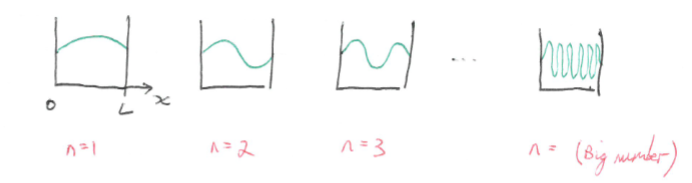
\includegraphics[width=0.8\textwidth]{figures/lec02-03.png}
     \caption{Possible cavity modes}
\end{figure}

The amplitude $a(x)$ can be given by this:
\[
    a(x) = \sin \left(\frac{n \pi x}{L}\right), n = 1, 2, 3, \ldots n \text{(mode number)}
\]

And by inspection from the figures:
\[
    \lambda = \frac{2L}{n}
\]

And therefore the number of nodes per wavelength is:
\[
    n(\lambda) = \frac{2L}{\lambda}
\]

So, classically:
\[
    I(\lambda) \propto \frac{n(\lambda)}{\lambda} \times k_B T \propto \frac{1}{\lambda^2}
\]

Where the first term is the density of nodes at lamda, and the second is the average energy of nodes. As we head to UV and $\lambda \to 0$, $I(\lambda) \to \infty$... which is not accurate. This is the UV Catastrophe!


\subsection*{Where did it go wrong?}
The issue was assuming that all cavity modes have average energy $k_B T$ - the ``Equipartition Theorem'' (which we'll meet in later courses).

In brief: the probability distribution of energies is a ``Boltzmann Distribution'':
\[
    p(E) = \frac{e^-{\frac{E}{k_B T}}}{k_B T}
\]

Average energy:
\[
    \bar{E} = \int_{0}^{\infty} E p (E) \, dE = k_B T
\]

Which seems to be incorrect...

\subsection*{Plank's Hypothesis}
A rather desperate Plank hypothesised that energy was quantised, i.e. it comes in discrete packets, called quanta. The energy of these quanta is proportional to frequency. This was radical at the time, even though we accept it now.

\[
    \Delta E = hf = \frac{hc}{\lambda}
\]
Where $h = 6.626 \times 10^{-34}Js$ is Plank's constant.

Sticking this into the Partition Function from statistical mechanics (which we will properly encounter later on, for now don't worry!), we get an average energy:
\[
    \bar{E}(\lambda) = \frac{hc/\lambda}{\exp(\lambda k_B T) - 1}
\]
Looking at limits:
\[
    \bar{E(\lambda \to \infty)}, \frac{hc}{\lambda k_BT} << 1
\]







    % !TeX root = main.tex
\lecture{3}{Thu 17 Oct 2025 12:00}{Particle Nature of Light}

In this lecture:
\begin{itemize}
    \item The photoelectric effect.
    \item Compton scattering.
\end{itemize}
Which are two examples where classical theory (light as a wave) break down.

\section*{The Photoelectric Effect}
When shining ultraviolet light on a metal surface, electrons are emitted. This is the photoelectric effect. 

Why are we not bombarded by electrons in daily life? For the electron to fly off, we must be in a vacuum. Otherwise, it'll immediately strike an air molecule and be absorbed.

\textbf{Photoelectric Effect Background}
\begin{itemize}
    \item Discovered by Hertz, 1887
    \item Thomson (1889) went further, so did Lenard (1902) and others.
    \item Einstein won his Nobel Prize for explaining this, not from relativity.
\end{itemize}

\begin{figure}[H]
    \centering
    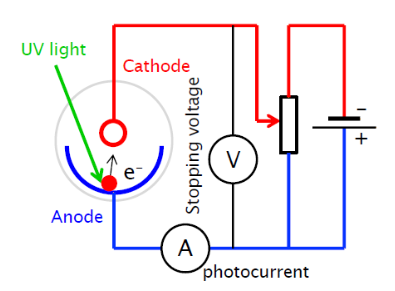
\includegraphics{figures/lec03-01.png}
     \caption{A circuit diagram for measuring the photoelectric effect.}
\end{figure}

The above setup would be encased in a glass ball (containing a vacuum), with a setup like this:

\begin{figure}[H]
    \centering
    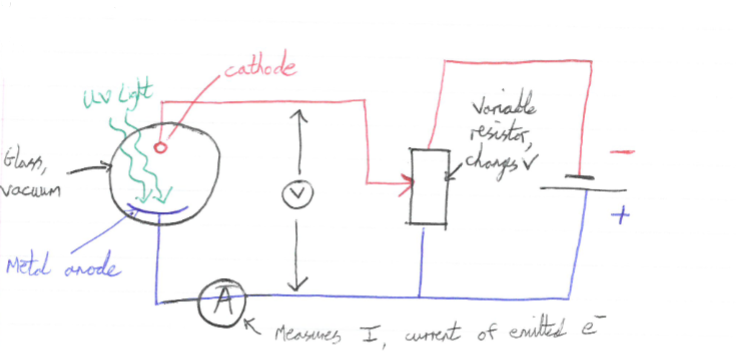
\includegraphics[width=0.75\textwidth]{figures/lec03-02.png}
     \caption{Experimental Setup}
\end{figure}

\subsection*{Results}
\textbf{Result One - Changing Intensity}\\
For fixed UV wavelength, increasing the intensity of light increases the measured photocurrent:
\begin{figure}[H]
    \centering
    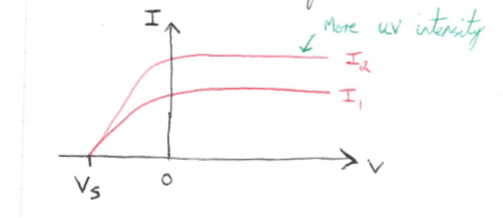
\includegraphics{figures/lec03-03.png}
    \caption{}
\end{figure}
\begin{itemize}
    \item Increasingly negative potential the cathode decreases photocurrent. At some potential $v_s$ (the ``stopping potential'') this current drops to zero.
    \item Potential does not affect electron emission, however adding potential causes an electric field which effectively blows electrons back towards the anode. The stopping potential is when this electric field is perfectly strong to prevent electrons from reaching the cathode and causing a current.
    \item The fact this can happen consistently (i.e. no current means no electrons made it through) implies that there must be some maximum kinetic energy these electrons can have ($KE_{max} = eV_S$).
    \item The stopping potential is independent of UV intensity. More UV makes current increase, but does not change stopping potential (i.e. it does not give more energy to each electron, they each have the same energy). This does not make sense classically. Classically we would expect adding more energy to cause emitted electrons to have more energy, therefore changing the stopping potential.
\end{itemize}

\textbf{Result Two - Changing Wavelength}
\begin{figure}[H]
    \centering
    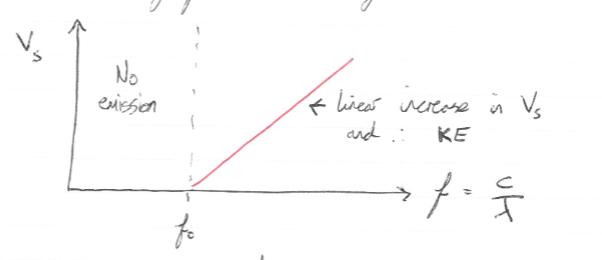
\includegraphics{figures/lec03-04.png}
    \caption{}
\end{figure}

We have to reach some baseline threshold frequency $f_0$ before we see any photocurrent. After this, increasing wavelength increases photocurrent (and hence KE of emitted electrons) linearly.

\begin{itemize}
    \item For a given metal, we find the threshold frequency $f_0$, below which there is no emission of electrons (no current). If below the frequency $f_0$, intensity is irrelevant. This contradicts classical mechanics which would suggest that turning up the light intensity would supply more (and potentially sufficient) energy.
    \item Above the threshold, the energy of individual emitted photons depends on UV frequency and not intensity (by result one).
\end{itemize}

\subsection*{Conclusions}

\textbf{Classically}

Classically, we expect energy to be proportional to intensity, $\therefore$ $v_s$ should increase with greater intensity. We also expect there to be no link between between frequency and energy, hence no threshold frequency. We'd expect no threshold frequency, instead being a time delay as electrons ``soak up'' energy to reach the required threshold.

In theory, great, in practice \emph{this is not observed.}

\textbf{Einstein's Proposal}

Energy in light comes from photons with energy $E = hf$. There is a minimum energy required for an electron to be able to escape from the metal. This minimum energy is called the work function $\phi$.
\[
    KE_\text{max} = hf - \phi = eV_s
\]

Now:
\begin{itemize}
    \item Higher intensity means more of the same particles (more photons), but the energy of each is unchanged.
    \item $E = hf$ so frequency changes energy (as observed).
    \item The Bohr model says that an electron can only have certain electron energy transitions when the correct energy is supplied (an electron cannot gradually soak up energy). This explains why there is a cutoff below the work function, and no observed time delay (as the ``soaking up'' that causes the delay does not happen). Either an incoming photon has sufficient energy, or it does not. Having more photons does not help.
    \item The first incoming photons immediately releases an electron (assuming the incoming light has sufficient energy), therefore there's no time delay.
\end{itemize}

\subsection*{In Practice}
\begin{figure}[H]
    \centering
    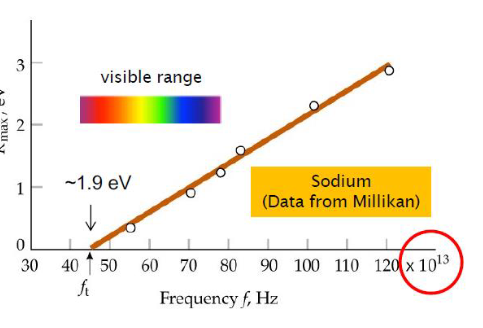
\includegraphics{figures/lec03-05.png}
     \caption{Sodium photocurrent measurements by Robert Millikan}
\end{figure}


\section*{Compton Scattering}
Compton Scattering is the scattering of x-rays off carbon atoms.

\begin{figure}[H]
    \centering
    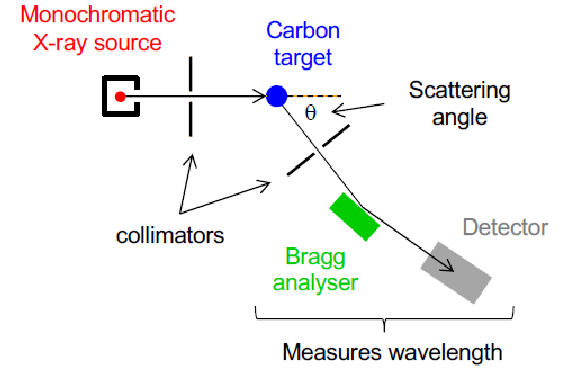
\includegraphics{figures/lec03-06.png}
     \caption{A Compton Scattering experimental setup.}
\end{figure}

The surprising result is that two wavelengths were observed (not just the original) - $\lambda_1, \lambda_2$, where $\lambda_1$ is the original and $\lambda_2$ is different. Classically this is hard to explain and $\lambda$ should not change.

The difference between these two wavelengths increases with scattering angle $\theta$. This can be explained if the x-ray beam is a stream of photons, but not classically.

Possible options when a photon collides:
\begin{itemize}
    \item Elastic: No loss of energy, hence no change in wavelength.
    \item Inelastic: Change of energy, so the wavelength also changes. An electron is fired out of the target, carrying energy and momentum, so the photon loses energy.
\end{itemize}

\begin{figure}[H]
    \centering
    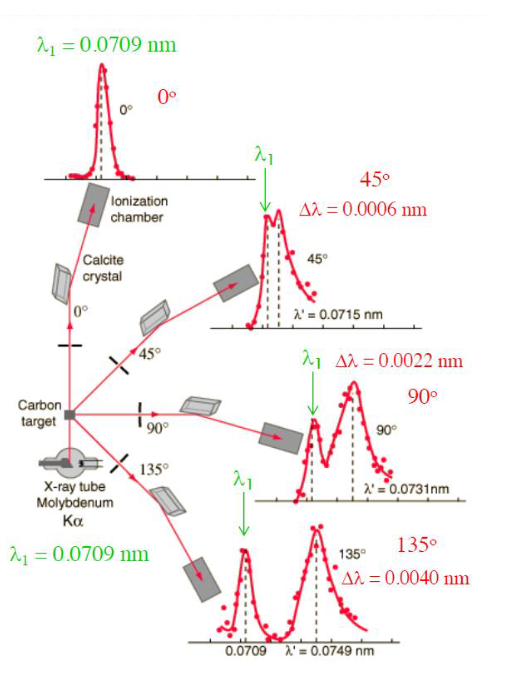
\includegraphics{figures/lec03-07.png}
     \caption{The observed results}
\end{figure}

\section*{Deriving Compton's Equation}
Given an incoming photon with with energy $E_1$, wavelength $\lambda_1$ and momentum $\underline{p}_1$. This strikes a carbon atom and is deflected by angle $\theta$. There is also an emitted electron at angle $\phi$ which must be in the opposite direction (angled up vs down) to conserve momentum. The new deflected photon has $E_2$, $\lambda_2$, $\underline{p}_2$.

We must consider relativistic effects here given the high speed ($E^2 = p^2c^2 + m^2c^4$)

\begin{figure}[H]
    \centering
    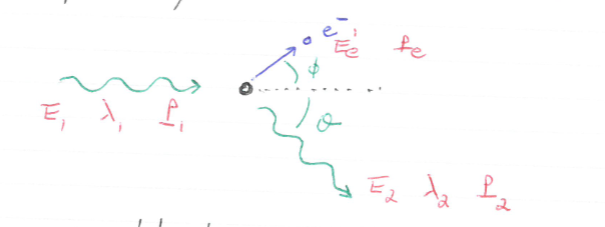
\includegraphics{figures/lec03-08.png}
     \caption{}
\end{figure}

\subsection*{Setup}
For a massless photon ($m = 0$):
\[
    E = pc
\]
And:
\[
    E = \frac{hc}{\lambda}
\]

So:
\begin{equation}
    p = \frac{h}{\lambda}
    \label{cscattere2}
\end{equation}

\subsection*{Conservation and Relativity}
Conserving momentum (underlines omitted for speed):
\[
    p_1 = p_e + p_2
\]
\[
    p_e = p_1 - p_2
\]

Squaring both sides:
\[
    p_e^2 = p_1^2 + p_2^2 - 2p_1 \cdot p_2
\]
\begin{equation}
    p_e^2 = p_1^2 + p_2^2 - 2p_1p_2 \cos \theta
    \label{cscattere1}    
\end{equation}

And then by conservation of energy:
\[
    E_1 + E_e = E_2 + E_e'
\]

Where $E_1$ is the incoming photon energy, $E_e$ is the energy of the electron at rest in atom before collision, $E_2$ is the deflected photon energy and finally $E_e'$ is the deflected electron's energy.

Using this:
\[
    p_1c + m_e c^2 = p_2 c + \sqrt{p_e^2c^2 + m_e^2c^4}
\]
\[
    \implies p_1 - p_2 + m_ec = \sqrt{p_e^2 + m_e^2c^2}
\]

And squaring both sides:
\[
    (p_1 - p_2)^2 + \cancel{m_e^2c^2} + 2m_ec(p_1 - p_2) = p_e^2 + \cancel{m_e^2c^2}
\]

Substituting in Eqn \ref{cscattere1} for $p_e^2$
\begin{align*}
    (p_1 - p_2)^2 + 2m_ec(p_1 - p_2) &= p_e^2\\
    (p_1 - p_2)^2 + 2m_ec(p_1 - p_2) &= p_1^2 + p_2^2 - 2p_1p_2 \cos \theta
\end{align*}

And rearranging:
\begin{align*}
    (p_1 - p_2)^2 + 2m_ec(p_1 - p_2) &= p_1^2 + p_2^2 - 2p_1p_2 \cos \theta\\
    p_1^2 + p_2^2 - 2p_1p_2 + 2m_ec(p_1 - p_2) &= p_1^2 + p_2^2 - 2p_1p_2 \cos \theta\\
    -2p_1p_2 + 2m_ec(p_1 - p_2) &= - 2p_1p_2 \cos \theta\\
    -p_1p_2 + m_ec(p_1 - p_2) &= - p_1p_2 \cos \theta\\
    m_ec(p_1 - p_2) &= - p_1p_2 \cos \theta + p_1p_2\\
    m_ec(p_1 - p_2) &= p_1p_2 (1 - \cos \theta) 
\end{align*}

Substituting Eqn \ref{cscattere2}:
\begin{align*}
    m_ec(p_1 - p_2) &= p_1p_2 (1 - \cos \theta)\\
    m_ec\left(\frac{h}{\lambda_1} - \frac{h}{\lambda_2}\right) &= \frac{h}{\lambda_1} \frac{h}{\lambda_2} (1 - \cos \theta)\\
    m_ec\left(\frac{h}{\lambda_1} - \frac{h}{\lambda_2}\right) &= \frac{h^2}{\lambda_1 \lambda_2} (1 - \cos \theta)\\
    m_ec\left(\frac{1}{\lambda_1} - \frac{1}{\lambda_2}\right) &= \frac{h}{\lambda_1 \lambda_2} (1 - \cos \theta)\\
    m_ec\left(\frac{\lambda_1 \lambda_2}{\lambda_1} - \frac{\lambda_1 \lambda_2}{\lambda_2}\right) &= h (1 - \cos \theta)\\
    m_ec\left(\lambda_2 - \lambda_1\right) &= h (1 - \cos \theta)\\
    \left(\lambda_2 - \lambda_1\right) &= \frac{h}{m_ec} (1 - \cos \theta)
\end{align*}

Which is the Compton Equation. This shows that the change in wavelength is proportional to $1 - \cos \theta$.

\section*{Conclusions}
The photoelectric effect and Compton scattering are two more physical phenomena that cannot be explained using traditional classical mechanics with EM waves alone. They both require assuming photons of energy $E = hf$ to be adequately explained.
    % end lectures CMR1

    \part*{LC Introduction to Probability and Statistics}
    \addcontentsline{toc}{part}{LC Introduction to Probability and Statistics}
    \graphicspath{{Introduction to Probability and Statistics/}}
    \course{LC Introduction to Probability and Statistics}
    % start lectures IPS
    % !TeX root = master.tex

\lecture{1}{Wed 01 Oct 2025 11:00}{Intro to Waves and SHM Recap}

\subsection*{Course Objectives}
\begin{itemize}
    \item Have a sound understanding of basic wave properties
    \item Have a basic understanding of interference effects, inc diffraction
    \item Be able to use simple geometric optics and understand the fundamentals of optical instruments.
\end{itemize}


\subsection*{Recommended Textbooks}
\begin{enumerate}
    \item University Physics, Young and Freedman (Ch 15, 16 for Waves, Ch 33-36 for Optics)
    \item Physics for Scientists and Engineers (Ch 20, 21 for Waves, Ch 22-24 for Optics)
    \item 5e, Tipler and Mosca, (Ch 15, 16 for Waves, 31-33 for Optics)
    \item Fundamentals of Optics, Jenkins and White
    \item Optics, Hecht and Zajac
\end{enumerate}

\paragraph{What is a wave?} Waves occur when a system is disturbed from equilibrian and the disturbance can travel from one region to another region. Waves carry energy, but do not move mass. The course aim is to derive basic equations for describing waves, and learn their physical properties.

\subsection*{Periodic Motion}
Waves are very linked to periodic motion. Therefore we recap periodic motion first.

It has these characterstics:
\begin{itemize}
    \item A period, $T$ (the time for one cycle)
    \item A frequency, $f$, the number of cycles per unit time ($f = \frac{1}{T}$)
    \item An amplitude, $A$, the maximum displacement from equilibrium.
\end{itemize}

Periodic motion continues due to the restoring force. When an object is displaced from equilibrium, the restoring force acts back towards the equi point. The object reaches equi with a non-zero speed, so the motion continues past the equi point and continues forever.

\subsection*{Energy}
Periodic motion is an exchange between potential and kinetic energy, with no energy loss. Energy is conserved.

\subsection*{Simple Harmonic Motion}
If the restoring force is directly proportional to the displacement $F = -kx$, then the periodic motion becomes Simple Harmonic Motion and the object is called a harmonic oscillator.

In a single dimension, displacement is given by:
\[
    x = A \cos(\omega t + \phi)
\]
Where $\omega = 2 \pi f$ is the angular velocity, and $\phi$ is the phase angle. In cases like this, where the phase angle is $90 \deg$ we can simplify to $x = A \cos(\omega t)$
\begin{figure}[H]
    \centering
    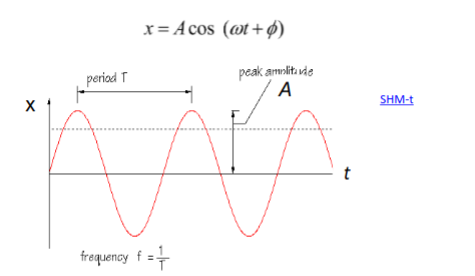
\includegraphics{figures/phaseangle.png}
    \caption{A Phase Angle of 90}
\end{figure}

\subsection*{More SHM Equations}
\textbf{Velocity}

\[
    v_x = \frac{dx}{dt} = - \omega A \sin(\omega t + \phi)
\]

\textbf{Acceleration}

\[
    a_x = \frac{d v_x}{dt} = \frac{d^2 x}{dt^2} = - \omega^2 A \cos(\omega t + \phi)
\]

Both properties are signed to indicate direction, as they are both vectors.




    % !TeX root = main.tex
\lecture{2}{Fri 10 Oct 2025 12:00}{The Ultraviolet Catastrophe}

In this lecture:
\begin{itemize}
    \item How classical theories fail to explain black body radiation (``The Ultraviolet Catastrophe'').
    \item How quantising light into photons gives predictions that fit this observation.
\end{itemize}

\section*{Black Body Radiation}
A `black body' is an idealised perfect object, that does not reflect, and absorbs internally all light (regardless of wavelength) incident upon it. No light is transmitted, so nothing shines out the other side. The object is perfectly black.

All bodies emit electromagnetic energy, usually outside the visible portion of the spectrum. For example, Paul Hollywood (and other humans) emit at about 300 Kelvin, which is infrared (at the temperature which night vision goggles are tuned to).

For the black body, emission spectrum is \textbf{only} from this thermal emission (no reflection, no flourescence, etc). Hotter objects are brighter and bluer (hotter means higher energy, and therefore a shorter wavelength)

\begin{figure}[H]
    \centering
    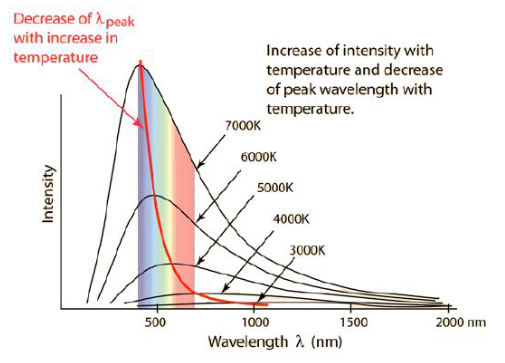
\includegraphics{figures/lec02-01.png}
     \caption{Observed Emission Spectra}
\end{figure}

However, we run into a problem. If we plot the spectra predicted by classical thermodynamics, vs the observed spectra for a given temperature object, the classical prediction gets it totally wrong, especially at shorter wavelengths.

\begin{figure}[H]
    \centering
    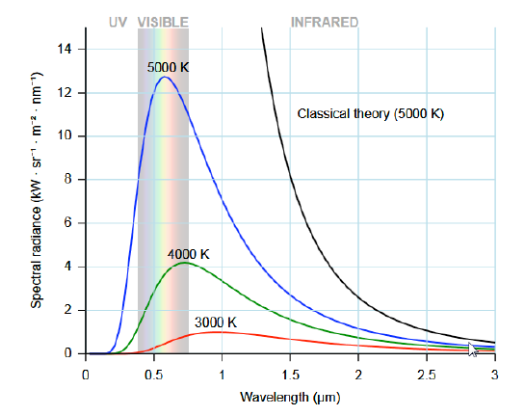
\includegraphics{figures/lec02-02.png}
     \caption{Predicted and Observed Spectra for 5000K (and Observed for 4k K and 3k K)}
\end{figure}

\subsection*{Notation}
$I(\lambda)$ is the intensity per wavelength for an emitted wavelength $\lambda$. $I$ is the total intensity across all wavelengths per unit time (in $W/m^2$, power per unit area).

\[
    I = \int_{0}^{\infty} I(\lambda) \, d \lambda
\]

I is the total area under the $I(\lambda)$ curve, i.e. the sum of intensity per wavelength, across every wavelength.

\section*{The Ultraviolet Catastrophe}
\subsection*{Empirical Results}
The Stefan-Boltzmann Law gives $I = \sigma T^4$, where $\sigma$ is the Stefan-Boltzmann constant, $\sigma = 6.57 \times 10^{-8} W m^{-2} K^{-4}$

Wien's Displacement Law gives $\lambda_{\text{peak}} = \frac{b}{T}$, where $b = 2.898 \times 10^{-3} Km$.

\subsection*{Why does classical mechanics break?}

Lets model the $I(\lambda)$ spectrum by slotting standing waves into a cavity. Consider a 1D cavity of length $L$. We can consider `cavity modes' as the possible waves that can exist in this cavity. As we know the wave is bound at each end, the displacement at each end of the cavity must be $0$. Therefore, the only possible waves must obey this, and these are cavity modes.

\begin{figure}[H]
    \centering
    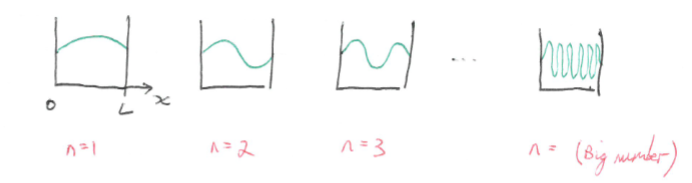
\includegraphics[width=0.8\textwidth]{figures/lec02-03.png}
     \caption{Possible cavity modes}
\end{figure}

The amplitude $a(x)$ can be given by this:
\[
    a(x) = \sin \left(\frac{n \pi x}{L}\right), n = 1, 2, 3, \ldots n \text{(mode number)}
\]

And by inspection from the figures:
\[
    \lambda = \frac{2L}{n}
\]

And therefore the number of nodes per wavelength is:
\[
    n(\lambda) = \frac{2L}{\lambda}
\]

So, classically:
\[
    I(\lambda) \propto \frac{n(\lambda)}{\lambda} \times k_B T \propto \frac{1}{\lambda^2}
\]

Where the first term is the density of nodes at lamda, and the second is the average energy of nodes. As we head to UV and $\lambda \to 0$, $I(\lambda) \to \infty$... which is not accurate. This is the UV Catastrophe!


\subsection*{Where did it go wrong?}
The issue was assuming that all cavity modes have average energy $k_B T$ - the ``Equipartition Theorem'' (which we'll meet in later courses).

In brief: the probability distribution of energies is a ``Boltzmann Distribution'':
\[
    p(E) = \frac{e^-{\frac{E}{k_B T}}}{k_B T}
\]

Average energy:
\[
    \bar{E} = \int_{0}^{\infty} E p (E) \, dE = k_B T
\]

Which seems to be incorrect...

\subsection*{Plank's Hypothesis}
A rather desperate Plank hypothesised that energy was quantised, i.e. it comes in discrete packets, called quanta. The energy of these quanta is proportional to frequency. This was radical at the time, even though we accept it now.

\[
    \Delta E = hf = \frac{hc}{\lambda}
\]
Where $h = 6.626 \times 10^{-34}Js$ is Plank's constant.

Sticking this into the Partition Function from statistical mechanics (which we will properly encounter later on, for now don't worry!), we get an average energy:
\[
    \bar{E}(\lambda) = \frac{hc/\lambda}{\exp(\lambda k_B T) - 1}
\]
Looking at limits:
\[
    \bar{E(\lambda \to \infty)}, \frac{hc}{\lambda k_BT} << 1
\]







    % end lectures IPS

    \part*{LC Mathematics for Physicists 1A}
    \addcontentsline{toc}{part}{LC Mathematics for Physicists 1A}
    \graphicspath{{Maths for Physicists 1A/}}
    \course{LC Mathematics for Physicists 1A}
    % start lectures MFP1A
    % !TeX root = master.tex

\lecture{1}{Wed 01 Oct 2025 11:00}{Intro to Waves and SHM Recap}

\subsection*{Course Objectives}
\begin{itemize}
    \item Have a sound understanding of basic wave properties
    \item Have a basic understanding of interference effects, inc diffraction
    \item Be able to use simple geometric optics and understand the fundamentals of optical instruments.
\end{itemize}


\subsection*{Recommended Textbooks}
\begin{enumerate}
    \item University Physics, Young and Freedman (Ch 15, 16 for Waves, Ch 33-36 for Optics)
    \item Physics for Scientists and Engineers (Ch 20, 21 for Waves, Ch 22-24 for Optics)
    \item 5e, Tipler and Mosca, (Ch 15, 16 for Waves, 31-33 for Optics)
    \item Fundamentals of Optics, Jenkins and White
    \item Optics, Hecht and Zajac
\end{enumerate}

\paragraph{What is a wave?} Waves occur when a system is disturbed from equilibrian and the disturbance can travel from one region to another region. Waves carry energy, but do not move mass. The course aim is to derive basic equations for describing waves, and learn their physical properties.

\subsection*{Periodic Motion}
Waves are very linked to periodic motion. Therefore we recap periodic motion first.

It has these characterstics:
\begin{itemize}
    \item A period, $T$ (the time for one cycle)
    \item A frequency, $f$, the number of cycles per unit time ($f = \frac{1}{T}$)
    \item An amplitude, $A$, the maximum displacement from equilibrium.
\end{itemize}

Periodic motion continues due to the restoring force. When an object is displaced from equilibrium, the restoring force acts back towards the equi point. The object reaches equi with a non-zero speed, so the motion continues past the equi point and continues forever.

\subsection*{Energy}
Periodic motion is an exchange between potential and kinetic energy, with no energy loss. Energy is conserved.

\subsection*{Simple Harmonic Motion}
If the restoring force is directly proportional to the displacement $F = -kx$, then the periodic motion becomes Simple Harmonic Motion and the object is called a harmonic oscillator.

In a single dimension, displacement is given by:
\[
    x = A \cos(\omega t + \phi)
\]
Where $\omega = 2 \pi f$ is the angular velocity, and $\phi$ is the phase angle. In cases like this, where the phase angle is $90 \deg$ we can simplify to $x = A \cos(\omega t)$
\begin{figure}[H]
    \centering
    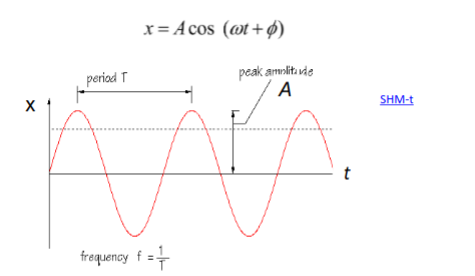
\includegraphics{figures/phaseangle.png}
    \caption{A Phase Angle of 90}
\end{figure}

\subsection*{More SHM Equations}
\textbf{Velocity}

\[
    v_x = \frac{dx}{dt} = - \omega A \sin(\omega t + \phi)
\]

\textbf{Acceleration}

\[
    a_x = \frac{d v_x}{dt} = \frac{d^2 x}{dt^2} = - \omega^2 A \cos(\omega t + \phi)
\]

Both properties are signed to indicate direction, as they are both vectors.




    % !TeX root = main.tex
\lecture{2}{Fri 10 Oct 2025 12:00}{The Ultraviolet Catastrophe}

In this lecture:
\begin{itemize}
    \item How classical theories fail to explain black body radiation (``The Ultraviolet Catastrophe'').
    \item How quantising light into photons gives predictions that fit this observation.
\end{itemize}

\section*{Black Body Radiation}
A `black body' is an idealised perfect object, that does not reflect, and absorbs internally all light (regardless of wavelength) incident upon it. No light is transmitted, so nothing shines out the other side. The object is perfectly black.

All bodies emit electromagnetic energy, usually outside the visible portion of the spectrum. For example, Paul Hollywood (and other humans) emit at about 300 Kelvin, which is infrared (at the temperature which night vision goggles are tuned to).

For the black body, emission spectrum is \textbf{only} from this thermal emission (no reflection, no flourescence, etc). Hotter objects are brighter and bluer (hotter means higher energy, and therefore a shorter wavelength)

\begin{figure}[H]
    \centering
    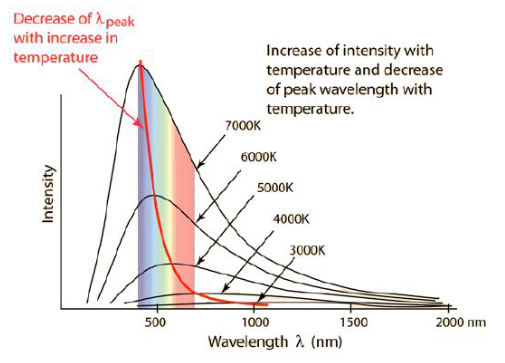
\includegraphics{figures/lec02-01.png}
     \caption{Observed Emission Spectra}
\end{figure}

However, we run into a problem. If we plot the spectra predicted by classical thermodynamics, vs the observed spectra for a given temperature object, the classical prediction gets it totally wrong, especially at shorter wavelengths.

\begin{figure}[H]
    \centering
    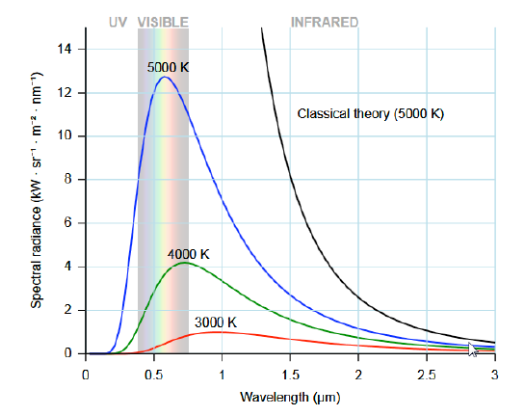
\includegraphics{figures/lec02-02.png}
     \caption{Predicted and Observed Spectra for 5000K (and Observed for 4k K and 3k K)}
\end{figure}

\subsection*{Notation}
$I(\lambda)$ is the intensity per wavelength for an emitted wavelength $\lambda$. $I$ is the total intensity across all wavelengths per unit time (in $W/m^2$, power per unit area).

\[
    I = \int_{0}^{\infty} I(\lambda) \, d \lambda
\]

I is the total area under the $I(\lambda)$ curve, i.e. the sum of intensity per wavelength, across every wavelength.

\section*{The Ultraviolet Catastrophe}
\subsection*{Empirical Results}
The Stefan-Boltzmann Law gives $I = \sigma T^4$, where $\sigma$ is the Stefan-Boltzmann constant, $\sigma = 6.57 \times 10^{-8} W m^{-2} K^{-4}$

Wien's Displacement Law gives $\lambda_{\text{peak}} = \frac{b}{T}$, where $b = 2.898 \times 10^{-3} Km$.

\subsection*{Why does classical mechanics break?}

Lets model the $I(\lambda)$ spectrum by slotting standing waves into a cavity. Consider a 1D cavity of length $L$. We can consider `cavity modes' as the possible waves that can exist in this cavity. As we know the wave is bound at each end, the displacement at each end of the cavity must be $0$. Therefore, the only possible waves must obey this, and these are cavity modes.

\begin{figure}[H]
    \centering
    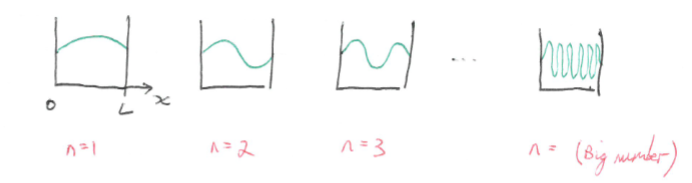
\includegraphics[width=0.8\textwidth]{figures/lec02-03.png}
     \caption{Possible cavity modes}
\end{figure}

The amplitude $a(x)$ can be given by this:
\[
    a(x) = \sin \left(\frac{n \pi x}{L}\right), n = 1, 2, 3, \ldots n \text{(mode number)}
\]

And by inspection from the figures:
\[
    \lambda = \frac{2L}{n}
\]

And therefore the number of nodes per wavelength is:
\[
    n(\lambda) = \frac{2L}{\lambda}
\]

So, classically:
\[
    I(\lambda) \propto \frac{n(\lambda)}{\lambda} \times k_B T \propto \frac{1}{\lambda^2}
\]

Where the first term is the density of nodes at lamda, and the second is the average energy of nodes. As we head to UV and $\lambda \to 0$, $I(\lambda) \to \infty$... which is not accurate. This is the UV Catastrophe!


\subsection*{Where did it go wrong?}
The issue was assuming that all cavity modes have average energy $k_B T$ - the ``Equipartition Theorem'' (which we'll meet in later courses).

In brief: the probability distribution of energies is a ``Boltzmann Distribution'':
\[
    p(E) = \frac{e^-{\frac{E}{k_B T}}}{k_B T}
\]

Average energy:
\[
    \bar{E} = \int_{0}^{\infty} E p (E) \, dE = k_B T
\]

Which seems to be incorrect...

\subsection*{Plank's Hypothesis}
A rather desperate Plank hypothesised that energy was quantised, i.e. it comes in discrete packets, called quanta. The energy of these quanta is proportional to frequency. This was radical at the time, even though we accept it now.

\[
    \Delta E = hf = \frac{hc}{\lambda}
\]
Where $h = 6.626 \times 10^{-34}Js$ is Plank's constant.

Sticking this into the Partition Function from statistical mechanics (which we will properly encounter later on, for now don't worry!), we get an average energy:
\[
    \bar{E}(\lambda) = \frac{hc/\lambda}{\exp(\lambda k_B T) - 1}
\]
Looking at limits:
\[
    \bar{E(\lambda \to \infty)}, \frac{hc}{\lambda k_BT} << 1
\]







    % !TeX root = main.tex
\lecture{3}{Thu 17 Oct 2025 12:00}{Particle Nature of Light}

In this lecture:
\begin{itemize}
    \item The photoelectric effect.
    \item Compton scattering.
\end{itemize}
Which are two examples where classical theory (light as a wave) break down.

\section*{The Photoelectric Effect}
When shining ultraviolet light on a metal surface, electrons are emitted. This is the photoelectric effect. 

Why are we not bombarded by electrons in daily life? For the electron to fly off, we must be in a vacuum. Otherwise, it'll immediately strike an air molecule and be absorbed.

\textbf{Photoelectric Effect Background}
\begin{itemize}
    \item Discovered by Hertz, 1887
    \item Thomson (1889) went further, so did Lenard (1902) and others.
    \item Einstein won his Nobel Prize for explaining this, not from relativity.
\end{itemize}

\begin{figure}[H]
    \centering
    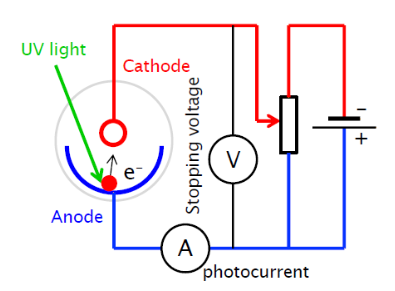
\includegraphics{figures/lec03-01.png}
     \caption{A circuit diagram for measuring the photoelectric effect.}
\end{figure}

The above setup would be encased in a glass ball (containing a vacuum), with a setup like this:

\begin{figure}[H]
    \centering
    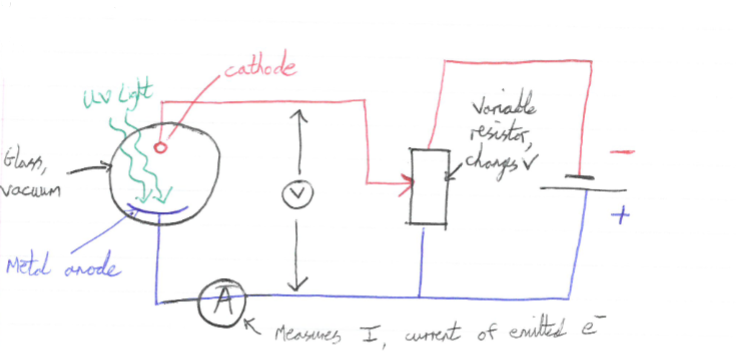
\includegraphics[width=0.75\textwidth]{figures/lec03-02.png}
     \caption{Experimental Setup}
\end{figure}

\subsection*{Results}
\textbf{Result One - Changing Intensity}\\
For fixed UV wavelength, increasing the intensity of light increases the measured photocurrent:
\begin{figure}[H]
    \centering
    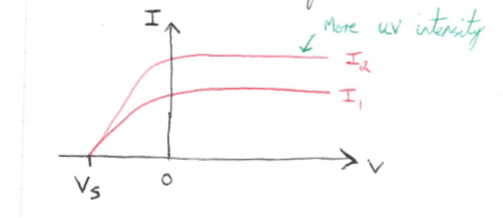
\includegraphics{figures/lec03-03.png}
    \caption{}
\end{figure}
\begin{itemize}
    \item Increasingly negative potential the cathode decreases photocurrent. At some potential $v_s$ (the ``stopping potential'') this current drops to zero.
    \item Potential does not affect electron emission, however adding potential causes an electric field which effectively blows electrons back towards the anode. The stopping potential is when this electric field is perfectly strong to prevent electrons from reaching the cathode and causing a current.
    \item The fact this can happen consistently (i.e. no current means no electrons made it through) implies that there must be some maximum kinetic energy these electrons can have ($KE_{max} = eV_S$).
    \item The stopping potential is independent of UV intensity. More UV makes current increase, but does not change stopping potential (i.e. it does not give more energy to each electron, they each have the same energy). This does not make sense classically. Classically we would expect adding more energy to cause emitted electrons to have more energy, therefore changing the stopping potential.
\end{itemize}

\textbf{Result Two - Changing Wavelength}
\begin{figure}[H]
    \centering
    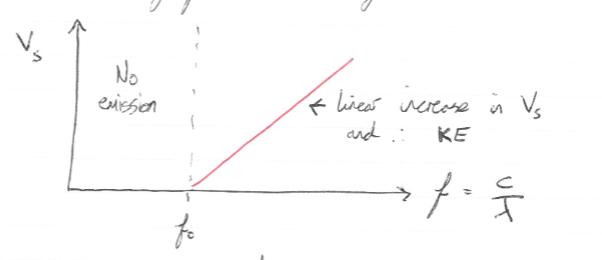
\includegraphics{figures/lec03-04.png}
    \caption{}
\end{figure}

We have to reach some baseline threshold frequency $f_0$ before we see any photocurrent. After this, increasing wavelength increases photocurrent (and hence KE of emitted electrons) linearly.

\begin{itemize}
    \item For a given metal, we find the threshold frequency $f_0$, below which there is no emission of electrons (no current). If below the frequency $f_0$, intensity is irrelevant. This contradicts classical mechanics which would suggest that turning up the light intensity would supply more (and potentially sufficient) energy.
    \item Above the threshold, the energy of individual emitted photons depends on UV frequency and not intensity (by result one).
\end{itemize}

\subsection*{Conclusions}

\textbf{Classically}

Classically, we expect energy to be proportional to intensity, $\therefore$ $v_s$ should increase with greater intensity. We also expect there to be no link between between frequency and energy, hence no threshold frequency. We'd expect no threshold frequency, instead being a time delay as electrons ``soak up'' energy to reach the required threshold.

In theory, great, in practice \emph{this is not observed.}

\textbf{Einstein's Proposal}

Energy in light comes from photons with energy $E = hf$. There is a minimum energy required for an electron to be able to escape from the metal. This minimum energy is called the work function $\phi$.
\[
    KE_\text{max} = hf - \phi = eV_s
\]

Now:
\begin{itemize}
    \item Higher intensity means more of the same particles (more photons), but the energy of each is unchanged.
    \item $E = hf$ so frequency changes energy (as observed).
    \item The Bohr model says that an electron can only have certain electron energy transitions when the correct energy is supplied (an electron cannot gradually soak up energy). This explains why there is a cutoff below the work function, and no observed time delay (as the ``soaking up'' that causes the delay does not happen). Either an incoming photon has sufficient energy, or it does not. Having more photons does not help.
    \item The first incoming photons immediately releases an electron (assuming the incoming light has sufficient energy), therefore there's no time delay.
\end{itemize}

\subsection*{In Practice}
\begin{figure}[H]
    \centering
    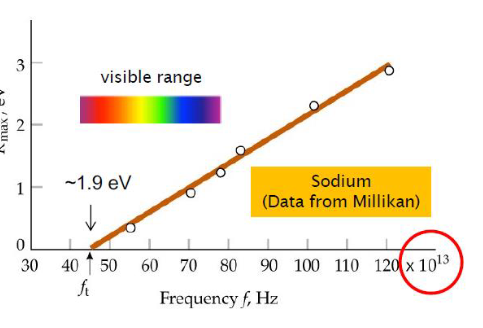
\includegraphics{figures/lec03-05.png}
     \caption{Sodium photocurrent measurements by Robert Millikan}
\end{figure}


\section*{Compton Scattering}
Compton Scattering is the scattering of x-rays off carbon atoms.

\begin{figure}[H]
    \centering
    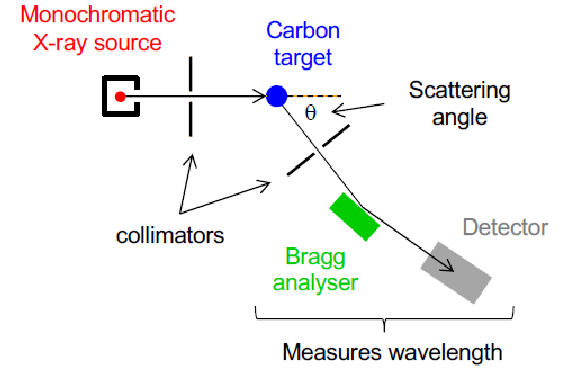
\includegraphics{figures/lec03-06.png}
     \caption{A Compton Scattering experimental setup.}
\end{figure}

The surprising result is that two wavelengths were observed (not just the original) - $\lambda_1, \lambda_2$, where $\lambda_1$ is the original and $\lambda_2$ is different. Classically this is hard to explain and $\lambda$ should not change.

The difference between these two wavelengths increases with scattering angle $\theta$. This can be explained if the x-ray beam is a stream of photons, but not classically.

Possible options when a photon collides:
\begin{itemize}
    \item Elastic: No loss of energy, hence no change in wavelength.
    \item Inelastic: Change of energy, so the wavelength also changes. An electron is fired out of the target, carrying energy and momentum, so the photon loses energy.
\end{itemize}

\begin{figure}[H]
    \centering
    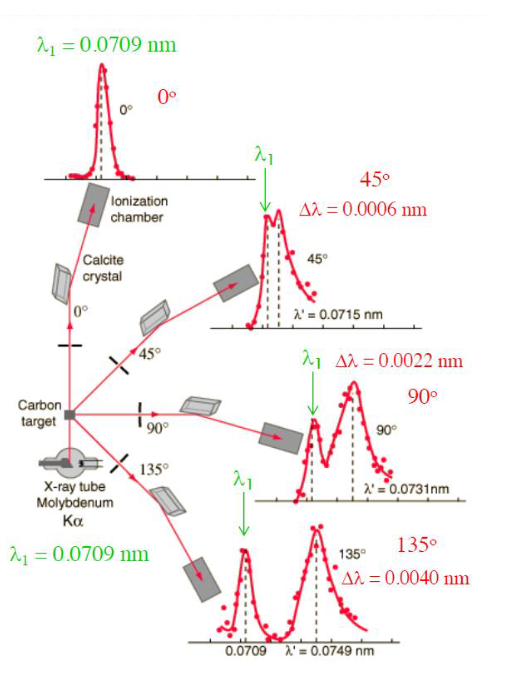
\includegraphics{figures/lec03-07.png}
     \caption{The observed results}
\end{figure}

\section*{Deriving Compton's Equation}
Given an incoming photon with with energy $E_1$, wavelength $\lambda_1$ and momentum $\underline{p}_1$. This strikes a carbon atom and is deflected by angle $\theta$. There is also an emitted electron at angle $\phi$ which must be in the opposite direction (angled up vs down) to conserve momentum. The new deflected photon has $E_2$, $\lambda_2$, $\underline{p}_2$.

We must consider relativistic effects here given the high speed ($E^2 = p^2c^2 + m^2c^4$)

\begin{figure}[H]
    \centering
    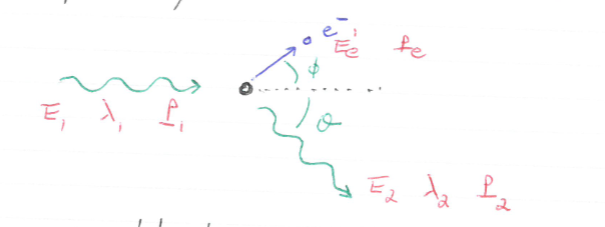
\includegraphics{figures/lec03-08.png}
     \caption{}
\end{figure}

\subsection*{Setup}
For a massless photon ($m = 0$):
\[
    E = pc
\]
And:
\[
    E = \frac{hc}{\lambda}
\]

So:
\begin{equation}
    p = \frac{h}{\lambda}
    \label{cscattere2}
\end{equation}

\subsection*{Conservation and Relativity}
Conserving momentum (underlines omitted for speed):
\[
    p_1 = p_e + p_2
\]
\[
    p_e = p_1 - p_2
\]

Squaring both sides:
\[
    p_e^2 = p_1^2 + p_2^2 - 2p_1 \cdot p_2
\]
\begin{equation}
    p_e^2 = p_1^2 + p_2^2 - 2p_1p_2 \cos \theta
    \label{cscattere1}    
\end{equation}

And then by conservation of energy:
\[
    E_1 + E_e = E_2 + E_e'
\]

Where $E_1$ is the incoming photon energy, $E_e$ is the energy of the electron at rest in atom before collision, $E_2$ is the deflected photon energy and finally $E_e'$ is the deflected electron's energy.

Using this:
\[
    p_1c + m_e c^2 = p_2 c + \sqrt{p_e^2c^2 + m_e^2c^4}
\]
\[
    \implies p_1 - p_2 + m_ec = \sqrt{p_e^2 + m_e^2c^2}
\]

And squaring both sides:
\[
    (p_1 - p_2)^2 + \cancel{m_e^2c^2} + 2m_ec(p_1 - p_2) = p_e^2 + \cancel{m_e^2c^2}
\]

Substituting in Eqn \ref{cscattere1} for $p_e^2$
\begin{align*}
    (p_1 - p_2)^2 + 2m_ec(p_1 - p_2) &= p_e^2\\
    (p_1 - p_2)^2 + 2m_ec(p_1 - p_2) &= p_1^2 + p_2^2 - 2p_1p_2 \cos \theta
\end{align*}

And rearranging:
\begin{align*}
    (p_1 - p_2)^2 + 2m_ec(p_1 - p_2) &= p_1^2 + p_2^2 - 2p_1p_2 \cos \theta\\
    p_1^2 + p_2^2 - 2p_1p_2 + 2m_ec(p_1 - p_2) &= p_1^2 + p_2^2 - 2p_1p_2 \cos \theta\\
    -2p_1p_2 + 2m_ec(p_1 - p_2) &= - 2p_1p_2 \cos \theta\\
    -p_1p_2 + m_ec(p_1 - p_2) &= - p_1p_2 \cos \theta\\
    m_ec(p_1 - p_2) &= - p_1p_2 \cos \theta + p_1p_2\\
    m_ec(p_1 - p_2) &= p_1p_2 (1 - \cos \theta) 
\end{align*}

Substituting Eqn \ref{cscattere2}:
\begin{align*}
    m_ec(p_1 - p_2) &= p_1p_2 (1 - \cos \theta)\\
    m_ec\left(\frac{h}{\lambda_1} - \frac{h}{\lambda_2}\right) &= \frac{h}{\lambda_1} \frac{h}{\lambda_2} (1 - \cos \theta)\\
    m_ec\left(\frac{h}{\lambda_1} - \frac{h}{\lambda_2}\right) &= \frac{h^2}{\lambda_1 \lambda_2} (1 - \cos \theta)\\
    m_ec\left(\frac{1}{\lambda_1} - \frac{1}{\lambda_2}\right) &= \frac{h}{\lambda_1 \lambda_2} (1 - \cos \theta)\\
    m_ec\left(\frac{\lambda_1 \lambda_2}{\lambda_1} - \frac{\lambda_1 \lambda_2}{\lambda_2}\right) &= h (1 - \cos \theta)\\
    m_ec\left(\lambda_2 - \lambda_1\right) &= h (1 - \cos \theta)\\
    \left(\lambda_2 - \lambda_1\right) &= \frac{h}{m_ec} (1 - \cos \theta)
\end{align*}

Which is the Compton Equation. This shows that the change in wavelength is proportional to $1 - \cos \theta$.

\section*{Conclusions}
The photoelectric effect and Compton scattering are two more physical phenomena that cannot be explained using traditional classical mechanics with EM waves alone. They both require assuming photons of energy $E = hf$ to be adequately explained.
    % end lectures MFP1A

    \part*{LC Optics and Waves}
    \addcontentsline{toc}{part}{LC Optics and Waves}
    \graphicspath{{Optics and Waves/}}
    \course{LC Optics and Waves}
    % start lectures OW
    % !TeX root = master.tex

\lecture{1}{Wed 01 Oct 2025 11:00}{Intro to Waves and SHM Recap}

\subsection*{Course Objectives}
\begin{itemize}
    \item Have a sound understanding of basic wave properties
    \item Have a basic understanding of interference effects, inc diffraction
    \item Be able to use simple geometric optics and understand the fundamentals of optical instruments.
\end{itemize}


\subsection*{Recommended Textbooks}
\begin{enumerate}
    \item University Physics, Young and Freedman (Ch 15, 16 for Waves, Ch 33-36 for Optics)
    \item Physics for Scientists and Engineers (Ch 20, 21 for Waves, Ch 22-24 for Optics)
    \item 5e, Tipler and Mosca, (Ch 15, 16 for Waves, 31-33 for Optics)
    \item Fundamentals of Optics, Jenkins and White
    \item Optics, Hecht and Zajac
\end{enumerate}

\paragraph{What is a wave?} Waves occur when a system is disturbed from equilibrian and the disturbance can travel from one region to another region. Waves carry energy, but do not move mass. The course aim is to derive basic equations for describing waves, and learn their physical properties.

\subsection*{Periodic Motion}
Waves are very linked to periodic motion. Therefore we recap periodic motion first.

It has these characterstics:
\begin{itemize}
    \item A period, $T$ (the time for one cycle)
    \item A frequency, $f$, the number of cycles per unit time ($f = \frac{1}{T}$)
    \item An amplitude, $A$, the maximum displacement from equilibrium.
\end{itemize}

Periodic motion continues due to the restoring force. When an object is displaced from equilibrium, the restoring force acts back towards the equi point. The object reaches equi with a non-zero speed, so the motion continues past the equi point and continues forever.

\subsection*{Energy}
Periodic motion is an exchange between potential and kinetic energy, with no energy loss. Energy is conserved.

\subsection*{Simple Harmonic Motion}
If the restoring force is directly proportional to the displacement $F = -kx$, then the periodic motion becomes Simple Harmonic Motion and the object is called a harmonic oscillator.

In a single dimension, displacement is given by:
\[
    x = A \cos(\omega t + \phi)
\]
Where $\omega = 2 \pi f$ is the angular velocity, and $\phi$ is the phase angle. In cases like this, where the phase angle is $90 \deg$ we can simplify to $x = A \cos(\omega t)$
\begin{figure}[H]
    \centering
    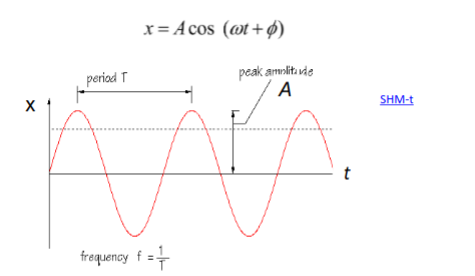
\includegraphics{figures/phaseangle.png}
    \caption{A Phase Angle of 90}
\end{figure}

\subsection*{More SHM Equations}
\textbf{Velocity}

\[
    v_x = \frac{dx}{dt} = - \omega A \sin(\omega t + \phi)
\]

\textbf{Acceleration}

\[
    a_x = \frac{d v_x}{dt} = \frac{d^2 x}{dt^2} = - \omega^2 A \cos(\omega t + \phi)
\]

Both properties are signed to indicate direction, as they are both vectors.




    % !TeX root = main.tex
\lecture{2}{Fri 10 Oct 2025 12:00}{The Ultraviolet Catastrophe}

In this lecture:
\begin{itemize}
    \item How classical theories fail to explain black body radiation (``The Ultraviolet Catastrophe'').
    \item How quantising light into photons gives predictions that fit this observation.
\end{itemize}

\section*{Black Body Radiation}
A `black body' is an idealised perfect object, that does not reflect, and absorbs internally all light (regardless of wavelength) incident upon it. No light is transmitted, so nothing shines out the other side. The object is perfectly black.

All bodies emit electromagnetic energy, usually outside the visible portion of the spectrum. For example, Paul Hollywood (and other humans) emit at about 300 Kelvin, which is infrared (at the temperature which night vision goggles are tuned to).

For the black body, emission spectrum is \textbf{only} from this thermal emission (no reflection, no flourescence, etc). Hotter objects are brighter and bluer (hotter means higher energy, and therefore a shorter wavelength)

\begin{figure}[H]
    \centering
    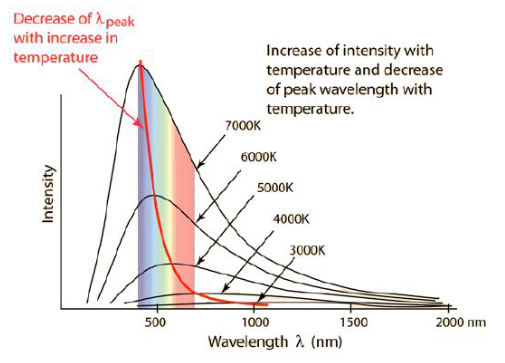
\includegraphics{figures/lec02-01.png}
     \caption{Observed Emission Spectra}
\end{figure}

However, we run into a problem. If we plot the spectra predicted by classical thermodynamics, vs the observed spectra for a given temperature object, the classical prediction gets it totally wrong, especially at shorter wavelengths.

\begin{figure}[H]
    \centering
    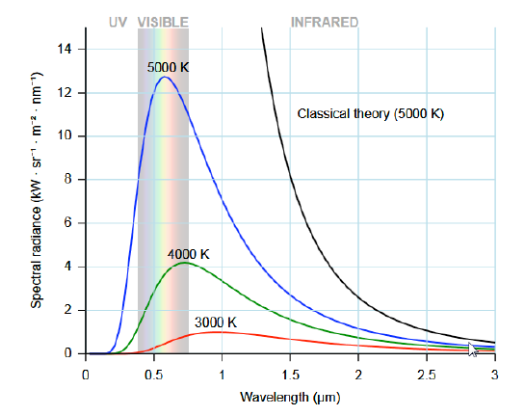
\includegraphics{figures/lec02-02.png}
     \caption{Predicted and Observed Spectra for 5000K (and Observed for 4k K and 3k K)}
\end{figure}

\subsection*{Notation}
$I(\lambda)$ is the intensity per wavelength for an emitted wavelength $\lambda$. $I$ is the total intensity across all wavelengths per unit time (in $W/m^2$, power per unit area).

\[
    I = \int_{0}^{\infty} I(\lambda) \, d \lambda
\]

I is the total area under the $I(\lambda)$ curve, i.e. the sum of intensity per wavelength, across every wavelength.

\section*{The Ultraviolet Catastrophe}
\subsection*{Empirical Results}
The Stefan-Boltzmann Law gives $I = \sigma T^4$, where $\sigma$ is the Stefan-Boltzmann constant, $\sigma = 6.57 \times 10^{-8} W m^{-2} K^{-4}$

Wien's Displacement Law gives $\lambda_{\text{peak}} = \frac{b}{T}$, where $b = 2.898 \times 10^{-3} Km$.

\subsection*{Why does classical mechanics break?}

Lets model the $I(\lambda)$ spectrum by slotting standing waves into a cavity. Consider a 1D cavity of length $L$. We can consider `cavity modes' as the possible waves that can exist in this cavity. As we know the wave is bound at each end, the displacement at each end of the cavity must be $0$. Therefore, the only possible waves must obey this, and these are cavity modes.

\begin{figure}[H]
    \centering
    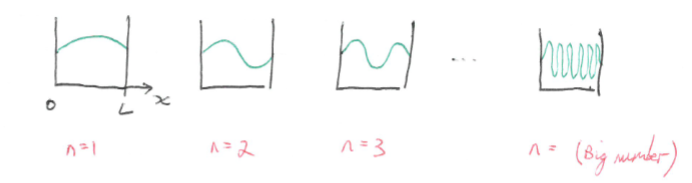
\includegraphics[width=0.8\textwidth]{figures/lec02-03.png}
     \caption{Possible cavity modes}
\end{figure}

The amplitude $a(x)$ can be given by this:
\[
    a(x) = \sin \left(\frac{n \pi x}{L}\right), n = 1, 2, 3, \ldots n \text{(mode number)}
\]

And by inspection from the figures:
\[
    \lambda = \frac{2L}{n}
\]

And therefore the number of nodes per wavelength is:
\[
    n(\lambda) = \frac{2L}{\lambda}
\]

So, classically:
\[
    I(\lambda) \propto \frac{n(\lambda)}{\lambda} \times k_B T \propto \frac{1}{\lambda^2}
\]

Where the first term is the density of nodes at lamda, and the second is the average energy of nodes. As we head to UV and $\lambda \to 0$, $I(\lambda) \to \infty$... which is not accurate. This is the UV Catastrophe!


\subsection*{Where did it go wrong?}
The issue was assuming that all cavity modes have average energy $k_B T$ - the ``Equipartition Theorem'' (which we'll meet in later courses).

In brief: the probability distribution of energies is a ``Boltzmann Distribution'':
\[
    p(E) = \frac{e^-{\frac{E}{k_B T}}}{k_B T}
\]

Average energy:
\[
    \bar{E} = \int_{0}^{\infty} E p (E) \, dE = k_B T
\]

Which seems to be incorrect...

\subsection*{Plank's Hypothesis}
A rather desperate Plank hypothesised that energy was quantised, i.e. it comes in discrete packets, called quanta. The energy of these quanta is proportional to frequency. This was radical at the time, even though we accept it now.

\[
    \Delta E = hf = \frac{hc}{\lambda}
\]
Where $h = 6.626 \times 10^{-34}Js$ is Plank's constant.

Sticking this into the Partition Function from statistical mechanics (which we will properly encounter later on, for now don't worry!), we get an average energy:
\[
    \bar{E}(\lambda) = \frac{hc/\lambda}{\exp(\lambda k_B T) - 1}
\]
Looking at limits:
\[
    \bar{E(\lambda \to \infty)}, \frac{hc}{\lambda k_BT} << 1
\]







    % end lectures OW

    \part*{LC Quantum Mechanics}
    \addcontentsline{toc}{part}{LC Quantum Mechanics}
    \graphicspath{{Quantum Mechanics/}}
    \course{LC Quantum Mechanics}
    % start lectures QM
    % !TeX root = master.tex

\lecture{1}{Wed 01 Oct 2025 11:00}{Intro to Waves and SHM Recap}

\subsection*{Course Objectives}
\begin{itemize}
    \item Have a sound understanding of basic wave properties
    \item Have a basic understanding of interference effects, inc diffraction
    \item Be able to use simple geometric optics and understand the fundamentals of optical instruments.
\end{itemize}


\subsection*{Recommended Textbooks}
\begin{enumerate}
    \item University Physics, Young and Freedman (Ch 15, 16 for Waves, Ch 33-36 for Optics)
    \item Physics for Scientists and Engineers (Ch 20, 21 for Waves, Ch 22-24 for Optics)
    \item 5e, Tipler and Mosca, (Ch 15, 16 for Waves, 31-33 for Optics)
    \item Fundamentals of Optics, Jenkins and White
    \item Optics, Hecht and Zajac
\end{enumerate}

\paragraph{What is a wave?} Waves occur when a system is disturbed from equilibrian and the disturbance can travel from one region to another region. Waves carry energy, but do not move mass. The course aim is to derive basic equations for describing waves, and learn their physical properties.

\subsection*{Periodic Motion}
Waves are very linked to periodic motion. Therefore we recap periodic motion first.

It has these characterstics:
\begin{itemize}
    \item A period, $T$ (the time for one cycle)
    \item A frequency, $f$, the number of cycles per unit time ($f = \frac{1}{T}$)
    \item An amplitude, $A$, the maximum displacement from equilibrium.
\end{itemize}

Periodic motion continues due to the restoring force. When an object is displaced from equilibrium, the restoring force acts back towards the equi point. The object reaches equi with a non-zero speed, so the motion continues past the equi point and continues forever.

\subsection*{Energy}
Periodic motion is an exchange between potential and kinetic energy, with no energy loss. Energy is conserved.

\subsection*{Simple Harmonic Motion}
If the restoring force is directly proportional to the displacement $F = -kx$, then the periodic motion becomes Simple Harmonic Motion and the object is called a harmonic oscillator.

In a single dimension, displacement is given by:
\[
    x = A \cos(\omega t + \phi)
\]
Where $\omega = 2 \pi f$ is the angular velocity, and $\phi$ is the phase angle. In cases like this, where the phase angle is $90 \deg$ we can simplify to $x = A \cos(\omega t)$
\begin{figure}[H]
    \centering
    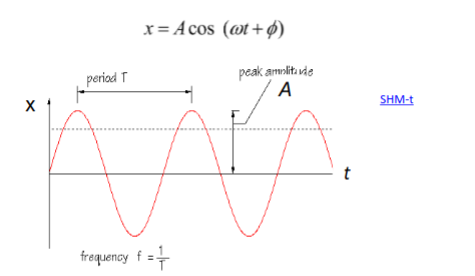
\includegraphics{figures/phaseangle.png}
    \caption{A Phase Angle of 90}
\end{figure}

\subsection*{More SHM Equations}
\textbf{Velocity}

\[
    v_x = \frac{dx}{dt} = - \omega A \sin(\omega t + \phi)
\]

\textbf{Acceleration}

\[
    a_x = \frac{d v_x}{dt} = \frac{d^2 x}{dt^2} = - \omega^2 A \cos(\omega t + \phi)
\]

Both properties are signed to indicate direction, as they are both vectors.




    % end lectures QM

\end{document}